\section{Исследование уравнения теплопроводности \label{heat}}
Целью данной главы является широкое рассмотрение подходов для решения нелинейных систем в одномерной, двумерной и трехмерной постановке.
Методы из главы \ref{methods} сравниваются, чтобы выбрать самые подходящие для решения системы функционала плотности. Сравнение проводится на упрощенной задаче \textemdash скалярном нелинейном уравнении теплопроводности. По аналогии с системой функционала плотности она включает в себя первую производную по времени и старшие производные по пространству с нелинейным коэффициентом.
\subsection{Постановка задачи}
Решается скалярное уравнение теплопроводности с нелинейным коэффициентом в кубической области $D \subset \mathbb{R^d}$, $t \in (0, T)$. Размерность пространства $d = \overline{1 \dots 3} $.
\begin{equation} \label{eq:heat_equation}
\frac{\partial u}{\partial t}+ \frac{\partial }{\partial x_i} \left( \alpha (u) \frac{\partial u}{\partial x_i} \right) = \nu(x_i, t)
\end{equation}
где $\nu(x_i, t)$ и $\alpha(u)$ - гладкие аналитические функции. Неизвестная функция $u(x_i, t)$ - гладкая.
\par
Задаются начальные условия:
\begin{equation} \label{eq:initial_condition_scalar}
u(x_i, t) \vert _{t = 0} = u_0(x_i)
\end{equation}
В качестве граничных условий рассматриваются \textit{условия Дирихле} или \textit{условия Неймана}:
\paragraph{условия Дирихле}
\begin{equation} \label{eq:dirichlet_heat}
u \vert_{\partial D} = \varphi(x_i, t)
\end{equation}
\paragraph{условия Неймана}
\begin{equation} \label{eq:neumann}
    \left. \frac{\partial u}{\partial n} \right \vert_{\partial D} = \varphi(x_i, t)
\end{equation}
где $n$ - вектор нормали к границе $\partial D$.
\subsection{Дискретизация}
Для аппроксимации производных по пространству пользуемся методом центральных разностей из раздела \ref{methods:space_derivative}. Таким образом, мы получаем 2-ой порядок аппроксимации по пространству. Рассмотрим, как этот порядок сохраняется в граничных точках.
\par
Границу области $D$ можно расположить по-разному относительно сетки в зависимости от граничных условий. Это позволяет избежать интерполяцию граничных условий и потерю точности. Разные варианты расположения границы показаны на рис. \ref{fig:heat_bound}. В случае \textit{граничных условий Дирихле} известно значение на границе. Поэтому удобно взять точку сетки на границе. В случае \textit{граничных условий Неймана} известна производная на границе. Можно аппроксимировать ее со вторым порядком. Для этого нужно взять две соседние точки сетки, равноудаленные от границы. 
\begin{figure}[H]
\centering
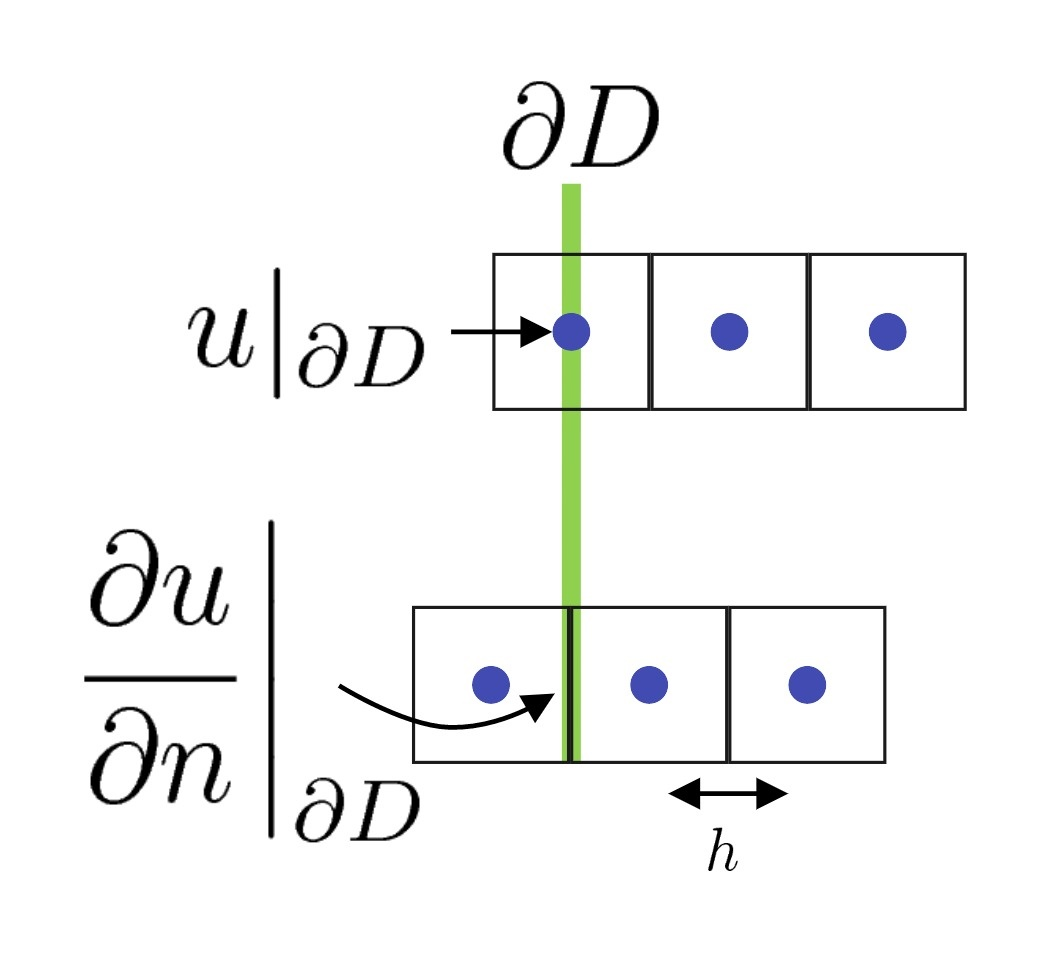
\includegraphics[width=.4\textwidth]{common_images/dirichlet_neumann.jpg}
\caption{Аппроксимация граничных условий. Синим цветом обозначены точки пространства, где ищется численное решение. Зеленым цветом обозначена граница.}
\label{fig:heat_bound}
\end{figure}
\subsection{Особенности реализации численных схем}
В рамках данной работы были реализованы программы, решающие уравнение теплопроводности \eqref{eq:heat_equation} в 1D, 2D и 3D. Поскольку реализовано большое количество похожих задач, отличающихся в деталях, сначала выпишем общие характеристики для всех решенных задач. Если не указано обратное, используется собственная реализация алгоритма.
Общие характеристики:
\begin{itemize}
\item Используем граничные условия Дирихле \eqref{eq:dirichlet_heat} и Неймана \eqref{eq:neumann}
\item Нелинейная система решается методом Ньютона (раздел \ref{methods:newton})
\item Отдельно реализованы линейная $\alpha(u) = const$ и нелинейная постановки задачи
\item Каждая задача решается явным и неявным по времени методом (раздел \ref{methods:time_integration})
\end{itemize}
Рассмотрим особенности реализации конкретных задач:
\paragraph{Одномерная задача}
\begin{itemize}
\item Неявное интегрирование по времени реализовано 3-мя способами: методом Эйлера, методом Кранка-Николсона и трехточечным методом второго порядка
\item Везде СЛАУ решается алгоритмом прогонки (раздел  \ref{methods:tridiagonal})
\item Система не предобуславливается
\end{itemize}

\paragraph{Двумерная задача}
\begin{itemize}
\item Кроме явной и неявной схемы, реализована схема переменных направлений (раздел \ref{methods:alternate_directions})
\item Предобуславливатель - метод ILU, реализация из Scipy (раздел \ref{methods:ilu})
\item Реализованы точный, численный и аналитический алгоритмы вычисления матрицы Якоби (раздел \ref{methods:computing_jacobi})
\end{itemize}

\paragraph{Трехмерная задача}
\begin{itemize}
\item Кроме явной и неявной схемы, реализована трехмерная схема переменных направлений, чтобы убедиться в ее неустойчивости
\item В неявном методе СЛАУ решается методом сопряженных градиентов
\item Предобуславливатель - разреженный метод LU (реализация из Scipy) и многосеточный метод (раздел \ref{methods:multigrid})
\item Расчет ведется на GPU с помощью PyCuda 
\end{itemize}
В двумерной и трехмерной постановках использовались не только указанные предобуславливатели, кроме них пробовались в качестве предобуславливателей все алгоритмы, описанные в главе \ref{methods}, однако вынесенные в список алгоритмы оказались наиболее производительными.

\subsubsection*{Особенность исследования сеточной сходимости}
Для правильной оценки нужно сравнивать значения в одни и те же моменты времени и в одних и тех же точках пространства. Поэтому более мелкие сетки должны точно проецироваться на самую крупную (рис. \ref{fig:convergence_bounds}). Для задачи с \textit{граничными условиями Дирихле} \eqref{eq:dirichlet_heat} шаг по пространству $h$ нужно делить в 2 раза, чтобы граничные точки попадали в себя. Для \textit{граничных условий Неймана} \eqref{eq:neumann} необходимо делить шаг по пространству в 3 раза. Первая точка находится на $\frac{h}{2}$ за границей, поэтому проецируется только внутренняя область.
\begin{figure}[H]
\centering
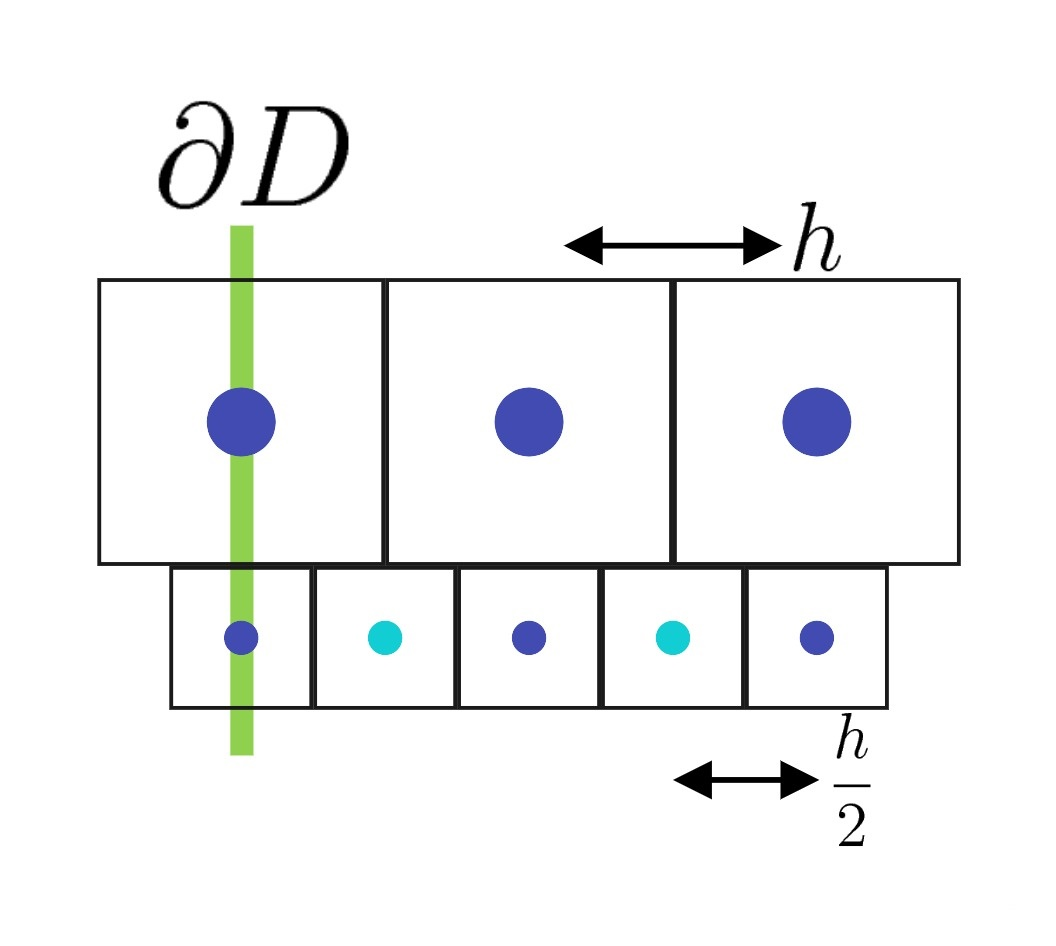
\includegraphics[width=.5\textwidth]{common_images/dividing_dirichlet.jpg}\hfill
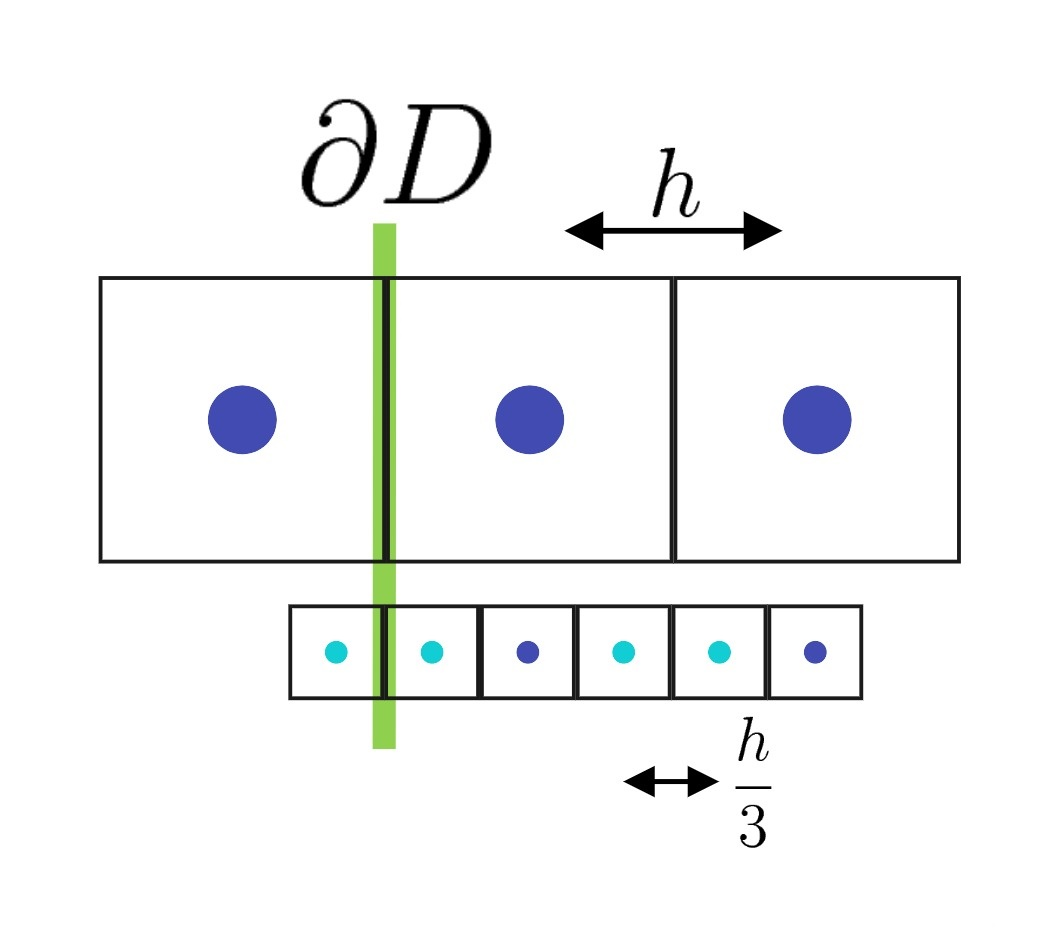
\includegraphics[width=.5\textwidth]{common_images/dividing_neumann.jpg}
\caption{Уменьшение сетки для граничных условий Дирихле (слева) и Неймана (справа). Темно-синим цветом выделены точки, проектирующиеся на более грубую сетку.}
\label{fig:convergence_bounds}
\end{figure}


\subsection{Численные эксперименты}
Исследование уравнения теплопроводности не является конечной целью данной работы. На его примере мы исследовали подходы, которые позже были использованы для более сложной системы функционала плотности. Поэтому все численные эксперименты с ним можно свести к исследованию корректности численных методов и их сходимости. Поскольку такие  эксперименты были проведены для каждой из описываемых задач, ограничимся приведением в данной работе только этих:
\begin{itemize}
\item Описание автоматического тестирования
\item Исследование сходимости метода переменных направлений в 2D
\item Сравнение результатов 2D и 3D расчетов
\item Исследование сходимости неявного метода в 3D
\end{itemize}
Для экспериментов, описанных ниже, используются граничные условия Дирихле. Задача решается в кубе $D = [0; 1]\times [0;1] \times [0;1]$, $t \in [0; 0.5]$. Мы формулируем постановку задачи на основе известной формулы, которая считается решением. Из нее вычисляются начальные и граничные условия, а также вычисляется вид источника. Во всех расчетах используется число Куранта:
\begin{equation}
\frac{\tau}{h^2} = 15
\end{equation}

\subsubsection{Автоматическое тестирование}
Для каждой задачи реализованы методы автоматического тестирования, описанные подробно в главе \ref{implementation:testing}:
\begin{itemize}
\item Сравнение линейной и нелинейной задачи
\item Тестирование операторов производной
\item Сравнение решения по разным методам для одной задачи
\end{itemize}

\subsubsection{Исследование сеточной сходимости 2D}
\paragraph{Постановка эксперимента}
В качестве решения используется формула:
\begin{equation}
u(x, y, t) = 2 + \sin \left(\pi \cdot \left( 0.5x + 0.25y - t\right) \right)
\end{equation}
В качестве нелинейного коэффициента используется:
\begin{equation}
\alpha(u) = \frac{u^{2} \left(\cos{\left(u \right)} + 2\right)}{9}
\end{equation}
Разобьем область по пространству и времени равномерными сетками. Минимальное количество точек в пространстве по каждому направлению - 21. Шаг по времени $\tau$ будем делить пропорционально $h^2$.

\paragraph{Применение символьной математики}
Если бы не действие нелинейного коэффициента $\alpha$, выбранное решение было бы собственной функцией для уравнения теплопроводности. Однако чтобы получить такое решение для нелинейного уравнения, источник должен постоянно действовать определенным образом. Чтобы найти вид источника, нужно подставить $\alpha$ и $u$ в уравнение теплопроводности. Выпишем вид источника, полученный с помощью символьной математики:
\begin{equation}
\begin{split}
\nu & (x, y, z, t) = 
\\ 
&- 0.0347222222222222 \pi^{2} \left(\sin{\left(\pi \left(- t + 0.5 x + 0.25 y\right) \right)} + 2\right)^{2}  \cdot 
\\ 
& \cdot \left(\cos{\left(\sin{\left(\pi \left(- t + 0.5 x + 0.25 y\right) \right)} + 2 \right)} + 2\right) \sin{\left(\pi \left(- t + 0.5 x + 0.25 y\right) \right)} -
\\
& -0.0347222222222222 \pi^{2} \left(\sin{\left(\pi \left(- t + 0.5 x + 0.25 y\right) \right)} + 2\right)^{2} \cdot 
\\
& \cdot  \sin{\left(\sin{\left(\pi \left(- t + 0.5 x + 0.25 y\right) \right)} + 2 \right)} \cos^{2}{\left(\pi \left(- t + 0.5 x + 0.25 y\right) \right)} +
\\
& + 0.0694444444444444 \pi^{2} \left(\sin{\left(\pi \left(- t + 0.5 x + 0.25 y\right) \right)} + 2\right)  \cdot
\\
& \cdot \left(\cos{\left(\sin{\left(\pi \left(- t + 0.5 x + 0.25 y\right) \right)} + 2 \right)} + 2\right) \cos^{2}{\left(\pi \left(- t + 0.5 x + 0.25 y\right) \right)} -
\\
& - \pi \cos{\left(\pi \left(- t + 0.5 x + 0.25 y\right) \right)}
\end{split}
\end{equation}

\paragraph{Результаты}
На рис. \ref{fig:heat2d_time_error} справа приведен график зависимости нормы ошибки от шага в последний момент времени задачи. Слева приведена зависимость нормы ошибки от времени. Везде используется норма $L_2$.
\begin{figure}[H]
\centering
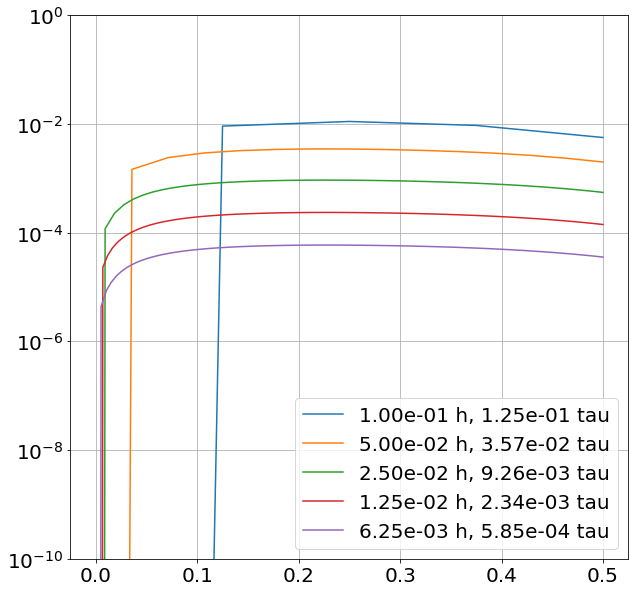
\includegraphics[width=.5\textwidth]{heat2d/time_error.png}\hfill
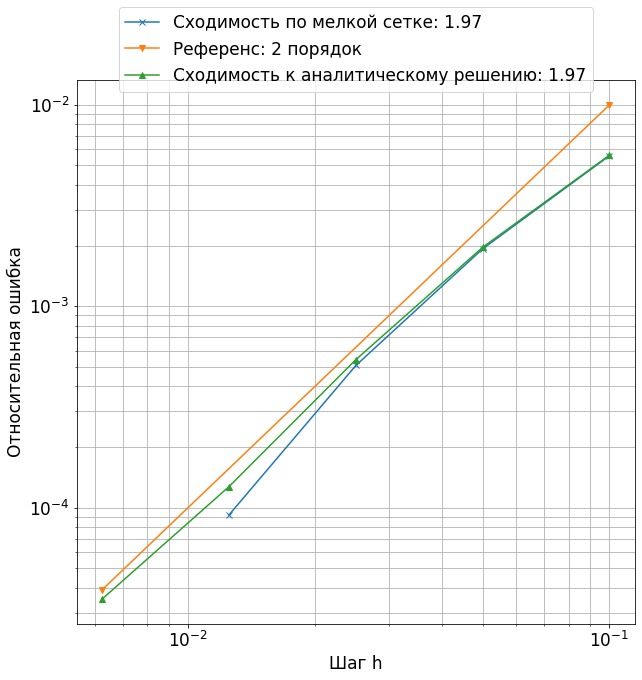
\includegraphics[width=.5\textwidth]{heat2d/convergence2d.png}
\caption{Зависимость нормы ошибки от времени (слева), зависимость нормы ошибки от шага сетки в последний момент расчета (справа)}
\label{fig:heat2d_time_error}
\end{figure}

Рассмотрим решения и ошибки в последний момент времени на рис. \ref{fig:heat2d_field}:

\begin{figure}[H]
\centering
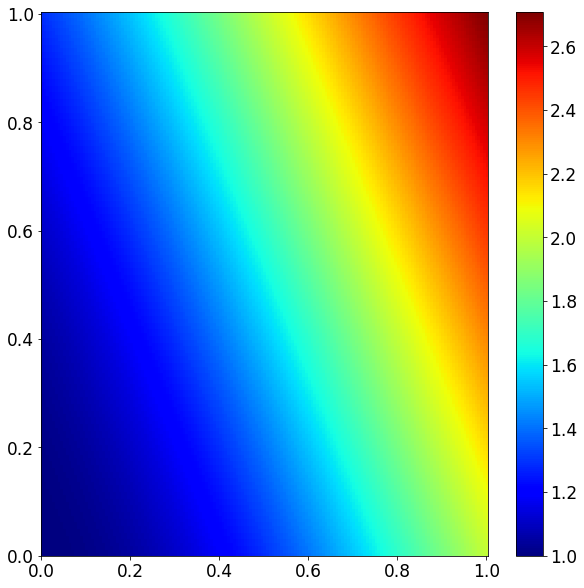
\includegraphics[height=.45\textwidth]{heat2d/solution.png}
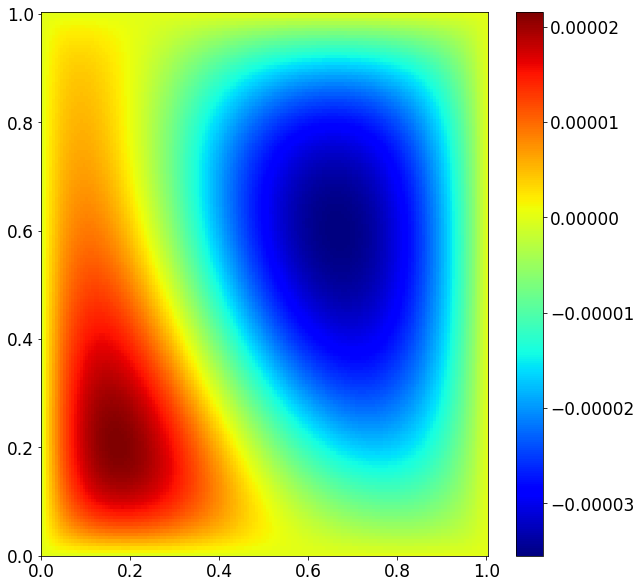
\includegraphics[height=.45\textwidth]{heat2d/error.png}
\caption{Решение (слева) и относительная ошибка (справа) на самой точной сетке из 161 точки по $x$ и $y$.}
\label{fig:heat2d_field}
\end{figure}



\subsubsection*{Сравнение результатов 2D и 3D расчетов}
Будем решать в трехмерной постановке двумерную задачу, как предложено в разделе \ref{implementation:testing}. Это позволит убедиться, что 2D и 3D расчеты согласованы и сходятся к одному и тому же решению.
\paragraph{Постановка численного эксперимента}
В качестве решения, из которого с помощью символьной математики ставится задача (раздел \ref{implementation:symbolic}), возьмем формулу:
\begin{equation}
u(x, y, t) = 2 + \sin \left(\pi \cdot \left( 0.5x + 0.25y - t\right) \right)
\end{equation}
В качестве нелинейного коэффициента возьмем:
\begin{equation}
\alpha(u) = \frac{u^2}{9}
\end{equation}
Двумерную задачу будем решать методом переменных направлений, а трехмерную - полностью неявным методом. Разобьем область равномерными сетками по пространству и времени. Для сеток по пространству используется 81 точка по каждому направлению. По времени пространство разбивается 215 точками.

\paragraph{Результаты} Проекцию по оси $z$ для сравнения берем посередине: $z = 0.5z_{max}$. 
Приведем графики решения 2D задачи и проекции решения 3D задачи на рис. \ref{fig:compare_2d_3d_fields}:
\begin{figure}[H]
\centering
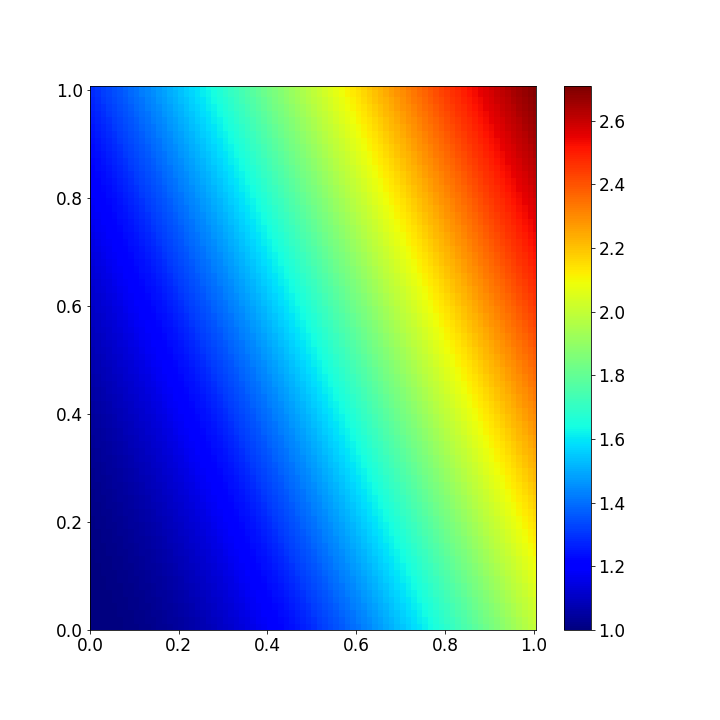
\includegraphics[width=.5\textwidth]{compare_2d_3d/field3d_80.png}\hfill
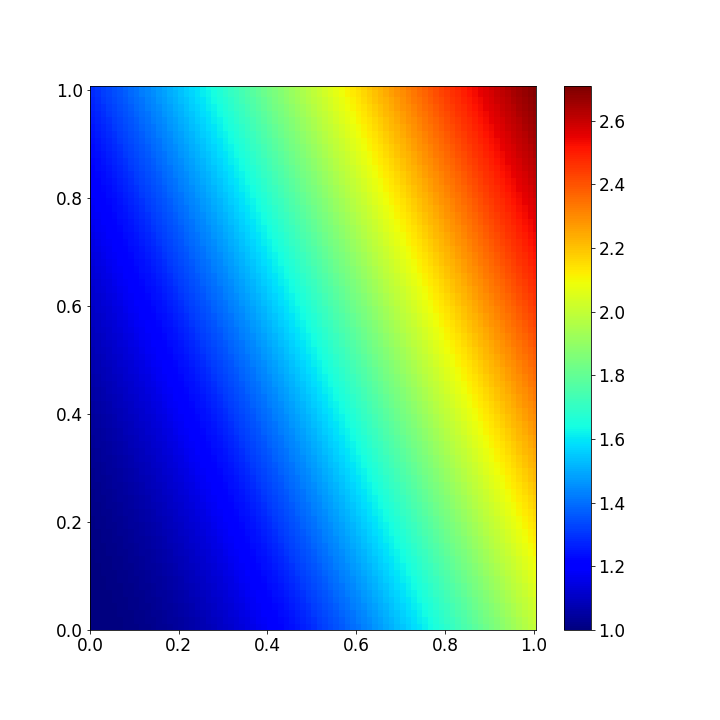
\includegraphics[width=.5\textwidth]{compare_2d_3d/field3d_80.png}
\caption{Проекция 3D решения (слева), 2D решение (справа)}
\label{fig:compare_2d_3d_fields}
\end{figure}
Визуально значения не отличаются. Построим разницу и сравним ее с ошибкой, полученной при сравнении с аналитическим решением на рис. \ref{fig:difference}:
\begin{figure}[H]
\centering
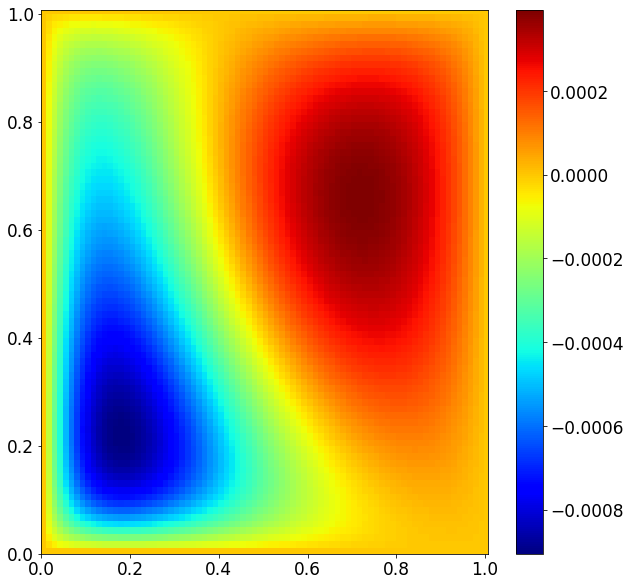
\includegraphics[width=.5\textwidth]{compare_2d_3d/difference.png}\hfill
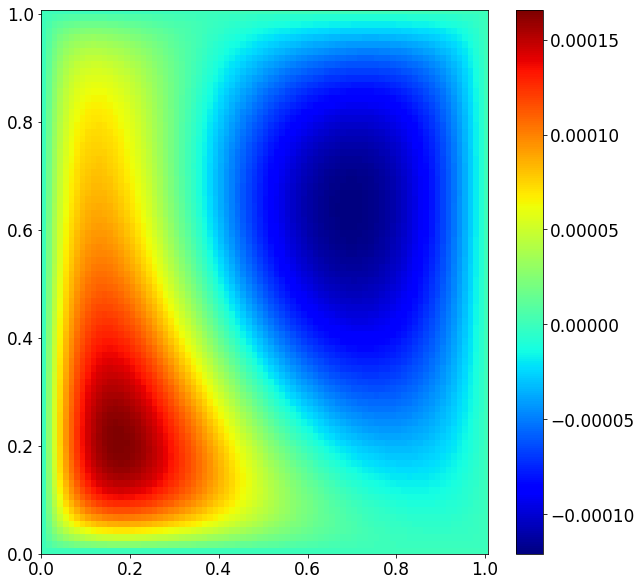
\includegraphics[width=.5\textwidth]{compare_2d_3d/error.png}
\caption{Разница между решениями 2D и 3D (слева), разница между аналитическим решением и 2D (справа)}
\label{fig:difference}
\end{figure}
По графикам видно, что разница между решениями, полученными разными методами, отражает значение реальной ошибки. Это позволяет исследовать порядок ошибки, не зная аналитического решения.

\subsubsection{Исследование сеточной сходимости неявной схемы в 3D \label{heat:convergence}}
Проведем исследование сходимости реализованного численно решения нелинейного уравнения теплопроводности в 3D с помощью методов из раздела \ref{implementation:convergence}
\paragraph{Постановка численного эксперимента}
Используем полностью неявную схему неявным методом Эйлера для аппроксимации производной по времени. Получим задачу теплопроводности из известного аналитического решения с помощью символьной математики (раздел \ref{implementation:symbolic}).
В качестве решения возьмем неотрицательную функцию:
\begin{equation}
u(x, y, z, t) = 2 + \sin \left(\pi \cdot \left( 0.5x + 0.25y + 0.75z - t\right) \right)
\end{equation}
В качестве нелинейного коэффициента возьмем:
\begin{equation}
\alpha(u) = \frac{u^2}{9}
\end{equation}

Минимальное количество точек по одной оси - 11, шаг $h$ уменьшается в 2 раза. Шаг по времени пропорционален $h^2$. Решим задачу на 4 сетках.
Выпишем вид источника, полученного с помощью символьной математики:

\begin{multline}
    \nu(x, y, z, t) = \\ - 0.0972 \pi^{2} \left(\sin{\left(\pi \left(- t + 0.5 x + 0.25 y + 0.75 z\right) \right)} + 2\right)^{2} \cdot \sin{\left(\pi \left(- t + 0.5 x + 0.25 y + 0.75 z\right) \right)} \\ + 0.194 \pi^{2} \left(\sin{\left(\pi \left(- t + 0.5 x + 0.25 y + 0.75 z\right) \right)} + 2\right) \cdot \cos^{2}{\left(\pi \left(- t + 0.5 x + 0.25 y + 0.75 z\right) \right)} \\ - \pi \cos{\left(\pi \left(- t + 0.5 x + 0.25 y + 0.75 z\right) \right)}
\end{multline}

\paragraph{Результаты расчета}
На рис. \ref{fig:heat3d_time_error} слева приведена зависимость нормы относительной $L_2$ ошибки от времени. Ошибка вычисляется как разность численного и аналитического решения во всем пространстве в конкретный момент времени. Справа зависимость нормы $L_2$ ошибки на последнем шаге расчета от шага сетки.

\begin{figure}[H]
\centering
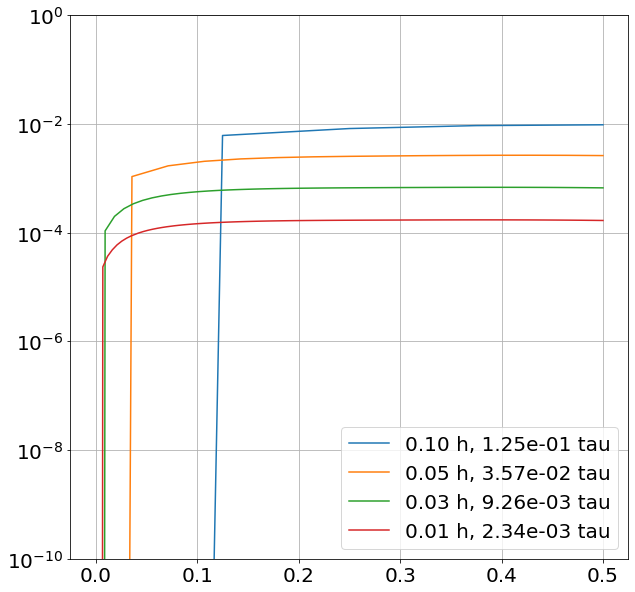
\includegraphics[width=.5\textwidth]{heat3d/time-error.png}\hfill
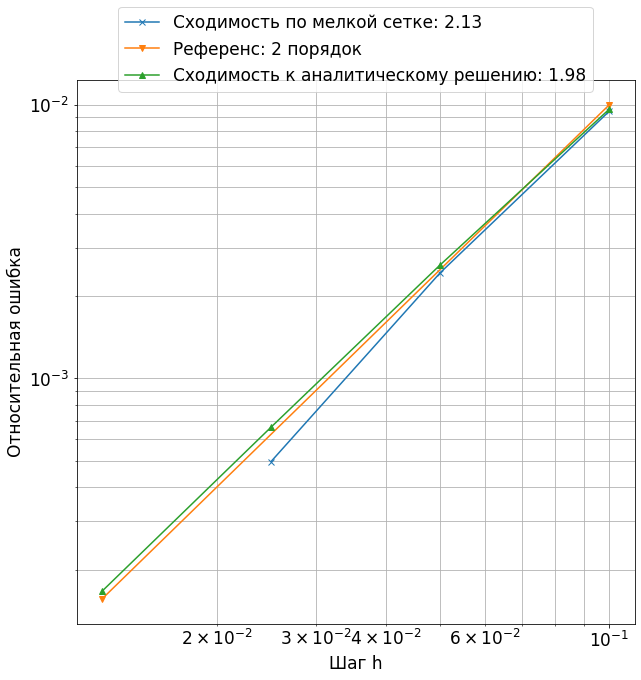
\includegraphics[width=.5\textwidth]{heat3d/convergence.png}
\caption{Зависимость нормы ошибки от времени (слева), зависимость нормы ошибки от шага сетки в последний момент расчета (справа)}
\label{fig:heat3d_time_error}
\end{figure}

Рассмотрим решения и ошибки на одной из 2D проекции расчетной области: $z = z_{max} / 2$ на рис. \ref{fig:heat3d_field}:

\begin{figure}[H]
\centering
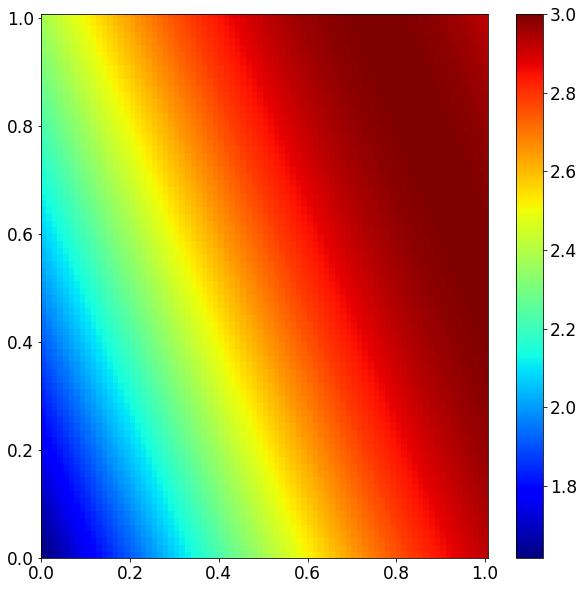
\includegraphics[height=.45\textwidth]{heat3d/solution_80dots.png}
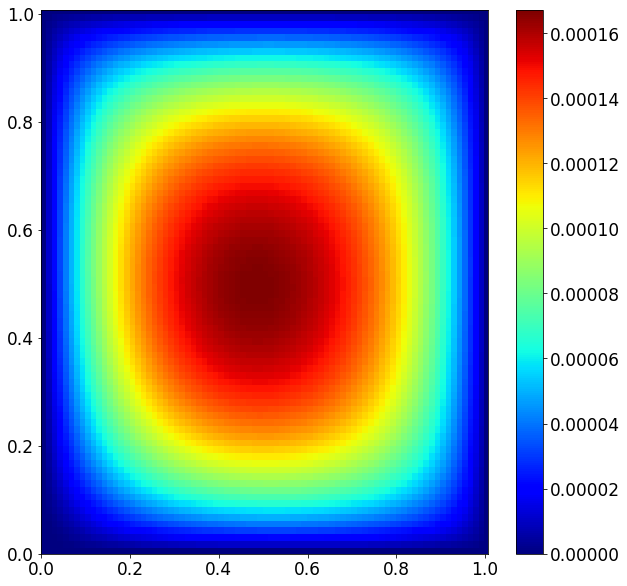
\includegraphics[height=.45\textwidth]{heat3d/rel_err_80dots.png}
\caption{Проекция $z=0.5z_{max}$: решение (слева) и относительная ошибка (справа)}
\label{fig:heat3d_field}
\end{figure}

\subsection{Вывод}
Подведем итог результатов, полученных в данной главе. Мы рассмотрели неявные по времени методы решения нелинейной задачи. В трехмерной постановке лучше всего себя зарекомендовала такая связка алгоритмов: полностью неявная схема, метод Ньютона для решения нелинейной системы, метод сопряженных градиентов для решения СЛАУ. Наиболее эффективным предобуславливателем был ILU и многосеточный метод. 
